\chapter{细胞因子}
\begin{framed}
\noindent\textbf{【知识体系】}
\begin{center}
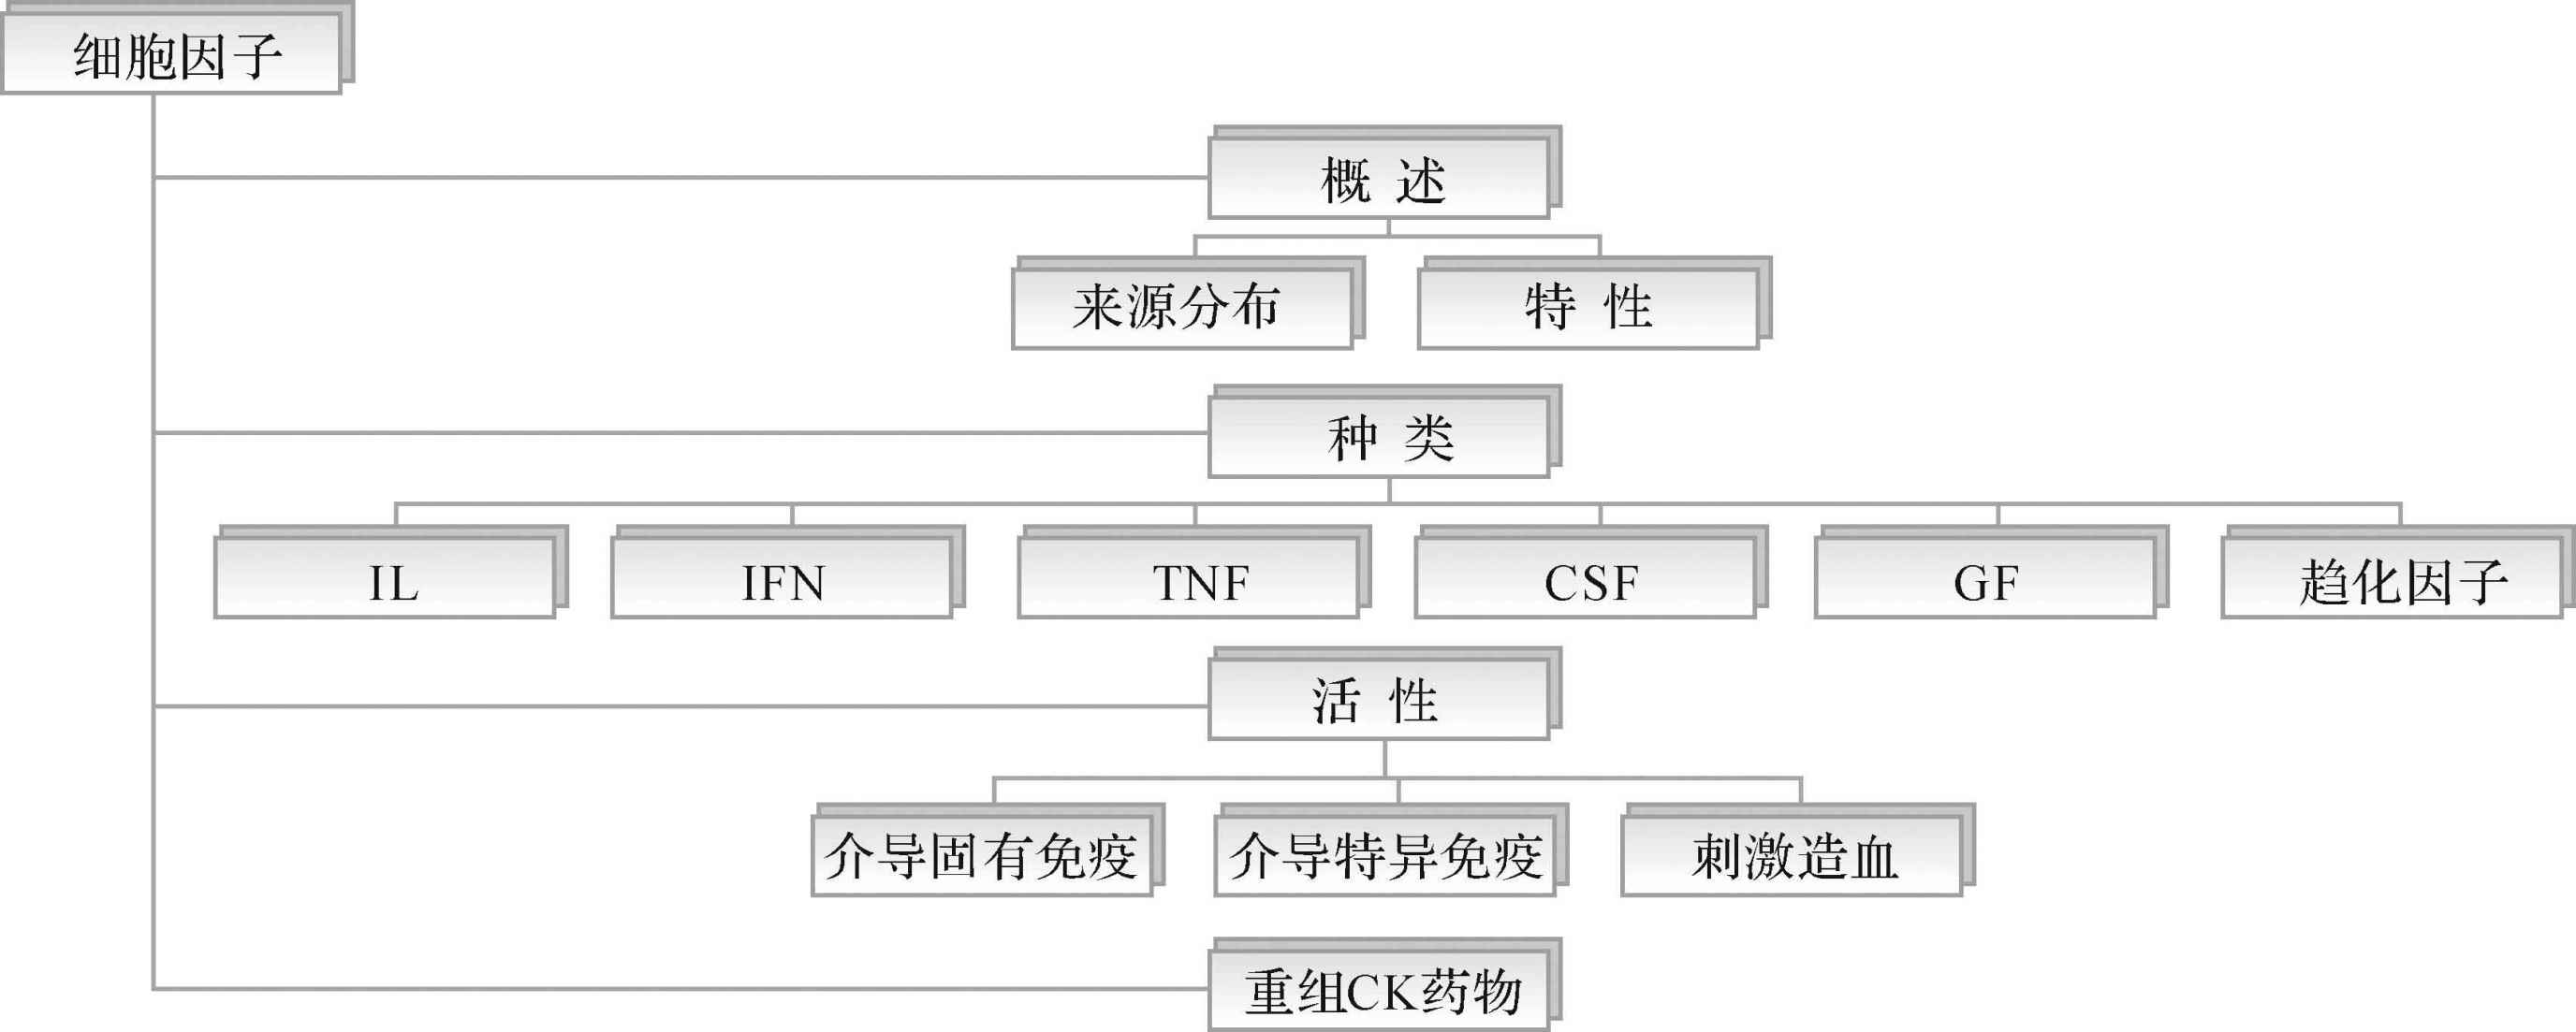
\includegraphics{./images/Image00090.jpg}
\end{center}
\noindent\textbf{【课前思考】}

为什么造血干细胞能分化为不同的细胞?B淋巴细胞为什么能分化为浆细胞分泌抗体?病毒入侵细胞时,细胞分泌什么物质抵御或抑制病毒?在免疫细胞分化发育、免疫调节、炎症反应、造血等功能中发挥调节作用的免疫分子是什么?有哪些特性?有多少种类?有什么生物学意义?

\noindent\textbf{【本章重点】}

1.细胞因子的概念、特性、种类;

2.细胞因子的生物学活性。

\noindent\textbf{【教学目标】}

1.掌握细胞因子的概念、共同特征,分泌方式;

2.掌握细胞因子分类(白细胞介素、干扰素、肿瘤坏死因子-α、集落刺激因子、生长因子、趋化性细胞因子);

3.熟悉细胞因子的生物学意义(抗菌、抗病毒、介导炎症反应,参与免疫应答和免疫调节,刺激造血等)。
\end{framed}

细胞因子(cytokine)是由多种细胞,特别是免疫细胞所产生、具有广泛生物学活性的小分子蛋白(分子量约8~80kD)。细胞因子在免疫细胞分化发育、免疫调节、炎症反应、造血功能中均发挥重要作用,并参与人体多种生理和病理过程的发生和发展。目前,已发现200余种人类细胞因子,随着人类基因组计划的完成,新的细胞因子家族及其成员将不断被发现。

\section{概述}


\subsection{细胞因子的来源和分布}

体内多种免疫细胞(如T细胞、B细胞、单核/巨噬细胞、NK细胞等)和非免疫细胞(如血管内皮细胞、表皮细胞、成纤维细胞等)均可产生细胞因子。此外,某些肿瘤细胞也可产生某些种类的细胞因子。多数细胞因子以单体形式存在,少数细胞因子如IL-10、IL-12、M-CSF、TGF-β等以双体形式存在,TNF可形成三聚体(图\ref{fig6-1})。

\begin{figure}[!htbp]
 \centering
 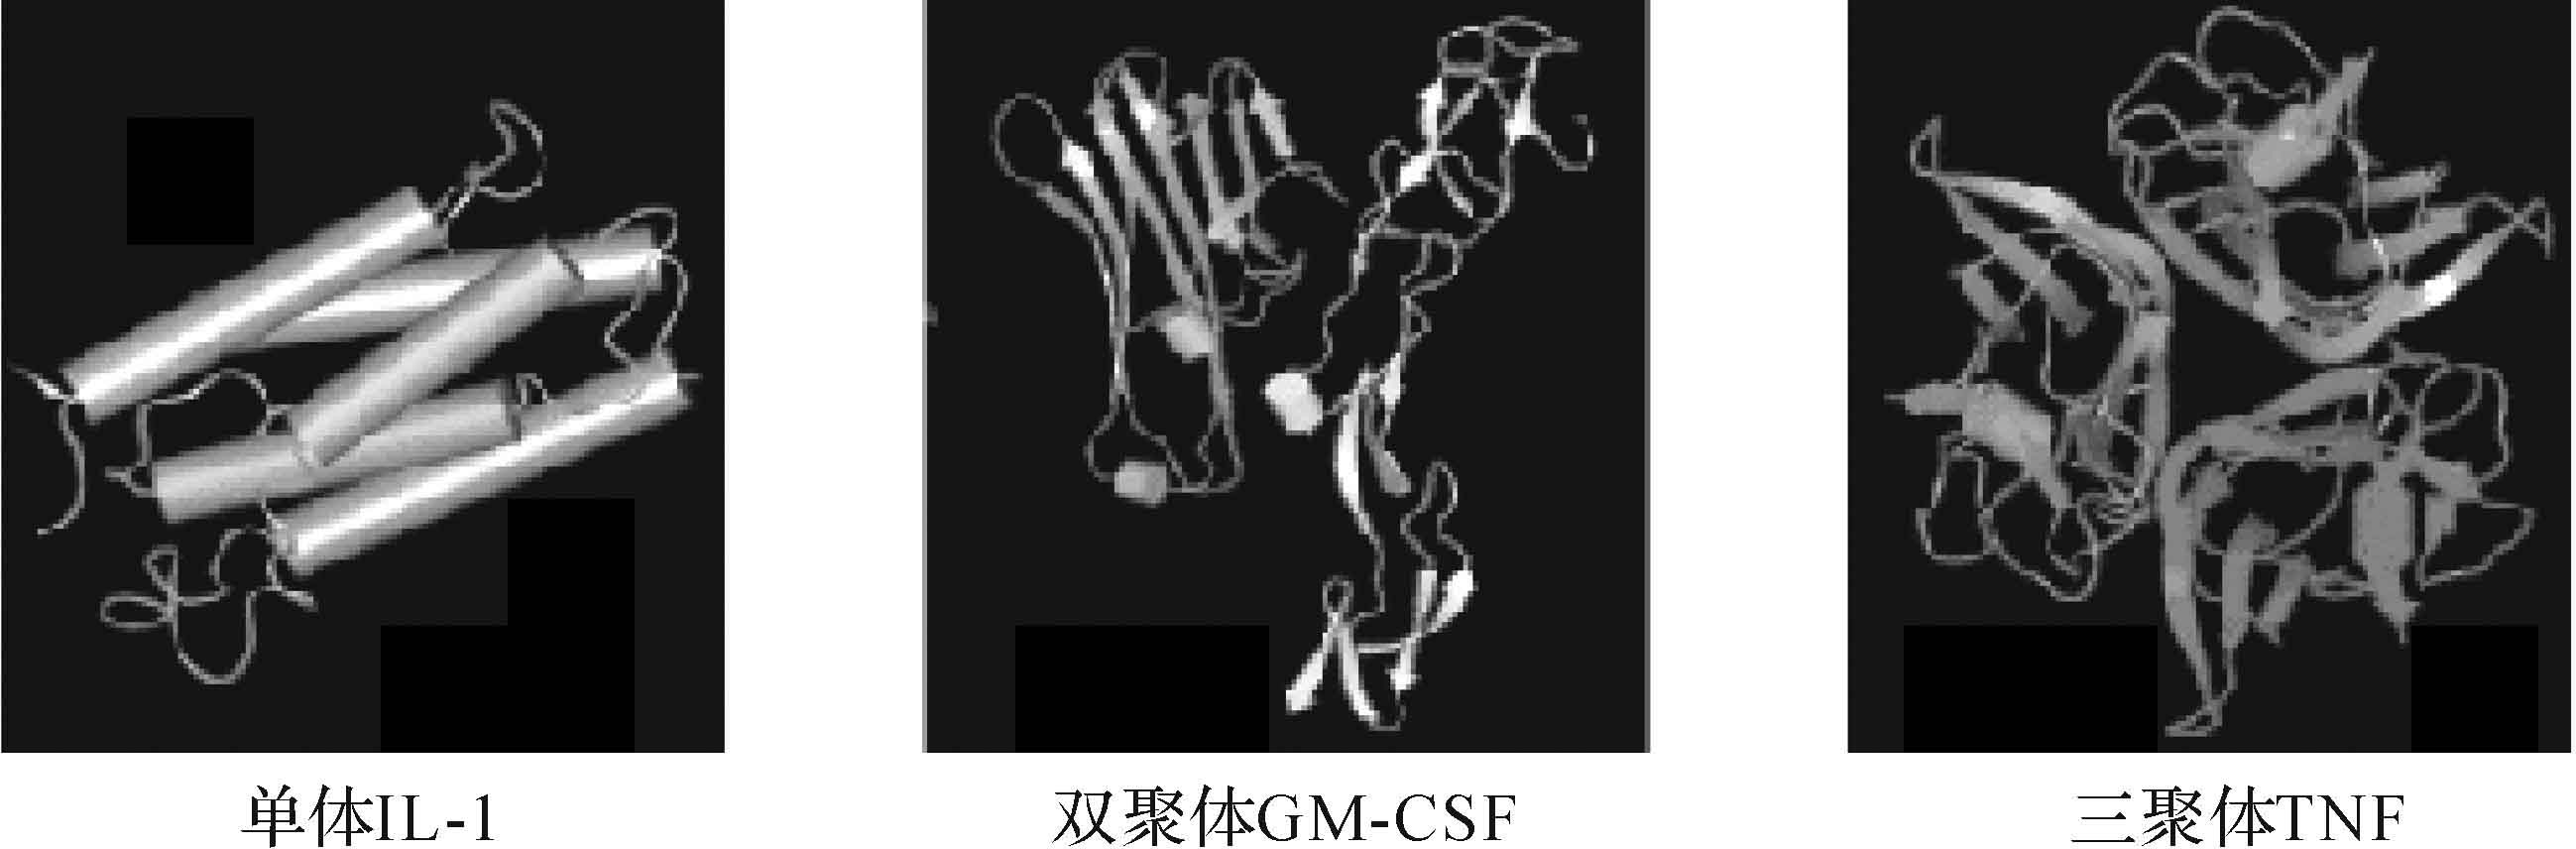
\includegraphics{./images/Image00091.jpg}
 \captionsetup{justification=centering}
 \caption{细胞因子的存在类型}
 \label{fig6-1}
  \end{figure} 

一般情况下,免疫细胞是细胞因子的主要来源,尤其是激活的淋巴细胞和单核/巨噬细胞可产生多种细胞因子。据此,可根据细胞因子的来源将其分为淋巴因子(lymphokine)和单核因子(monokine)。前者包括IL-2、IL-4、IL-5、IFN等;后者包括TNF-a、IL-1、IL-6、IL-8等。

多数细胞因子是以可溶性蛋白的形式分布于组织间质和体液中,但某些细胞因子(如TNF等)可以跨膜分子形式表达于产生细胞的表面。


\subsection{细胞因子的一般特性}

1.均为低分子量的多肽或糖蛋白。分子量约6~60 KD,少于200氨基酸。

2.细胞因子的产生具有:

多向性:一种淋巴细胞产生多种CKs。

多源性:多种细胞产生一种CKs。

3.与相应受体特异性结合才能发挥作用。细胞因子可以旁分泌、自分泌或内分泌的方式发挥作用(图\ref{fig6-2})。

\begin{figure}[!htbp]
 \centering
 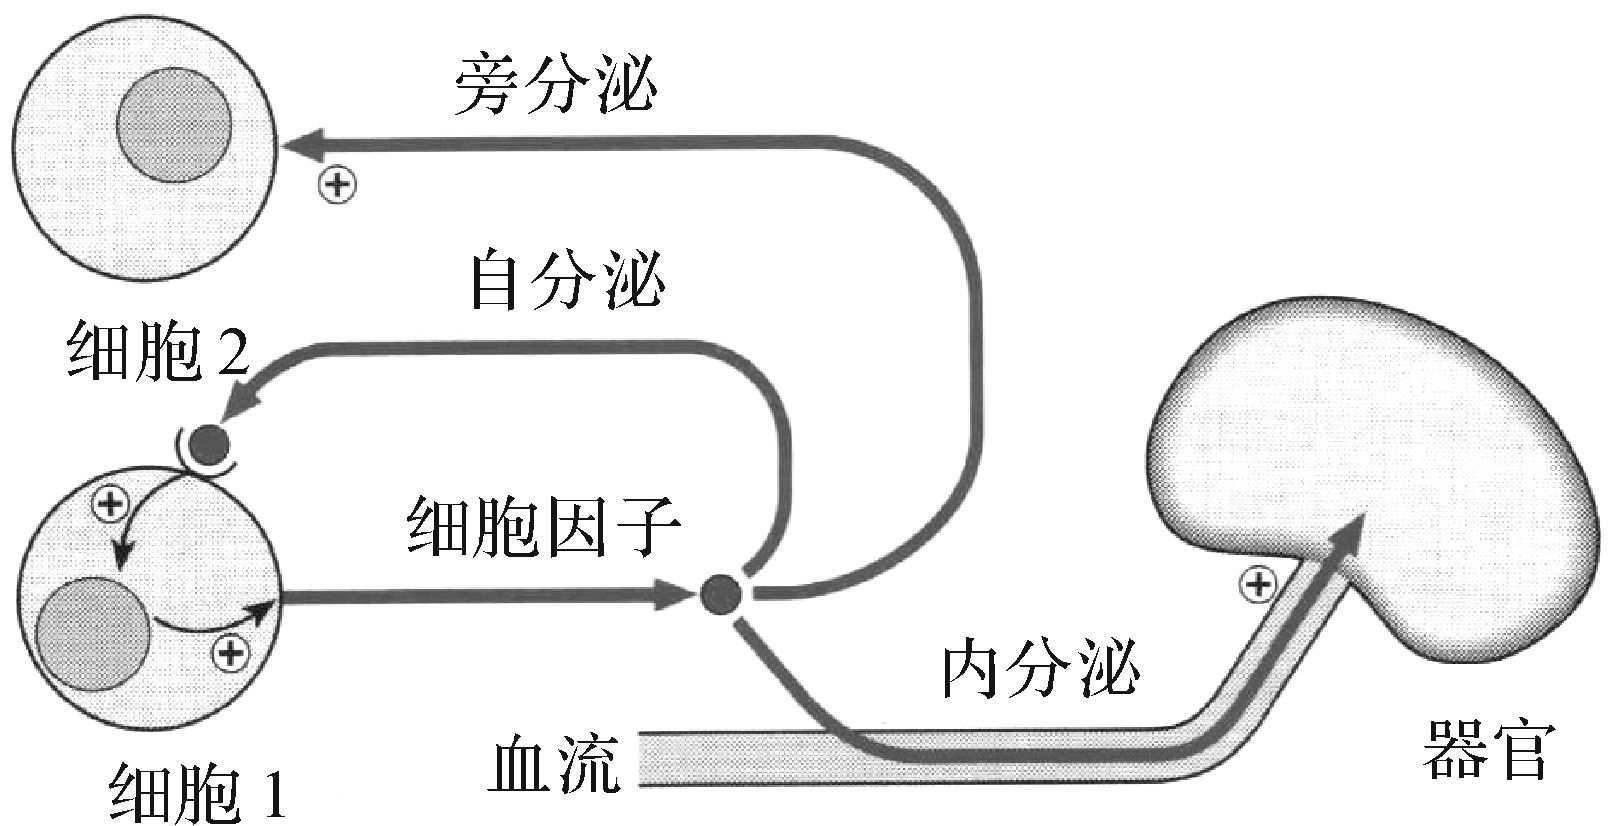
\includegraphics{./images/Image00092.jpg}
 \captionsetup{justification=centering}
 \caption{细胞因子的作用方式}
 \label{fig6-2}
  \end{figure} 

4.具有高效性、多效性、网络性。

(1)高效性:在10\textsuperscript{-10} ~10\textsuperscript{-15}
mol就能发挥作用。

(2)多效性:一种CKs 产生多种生物学效应。

(3)网络性:CKs相互渗透,调节细胞的活化与分化,表现增强或抑制,具有免疫调节作用(图\ref{fig6-3})。

\begin{figure}[!htbp]
 \centering
 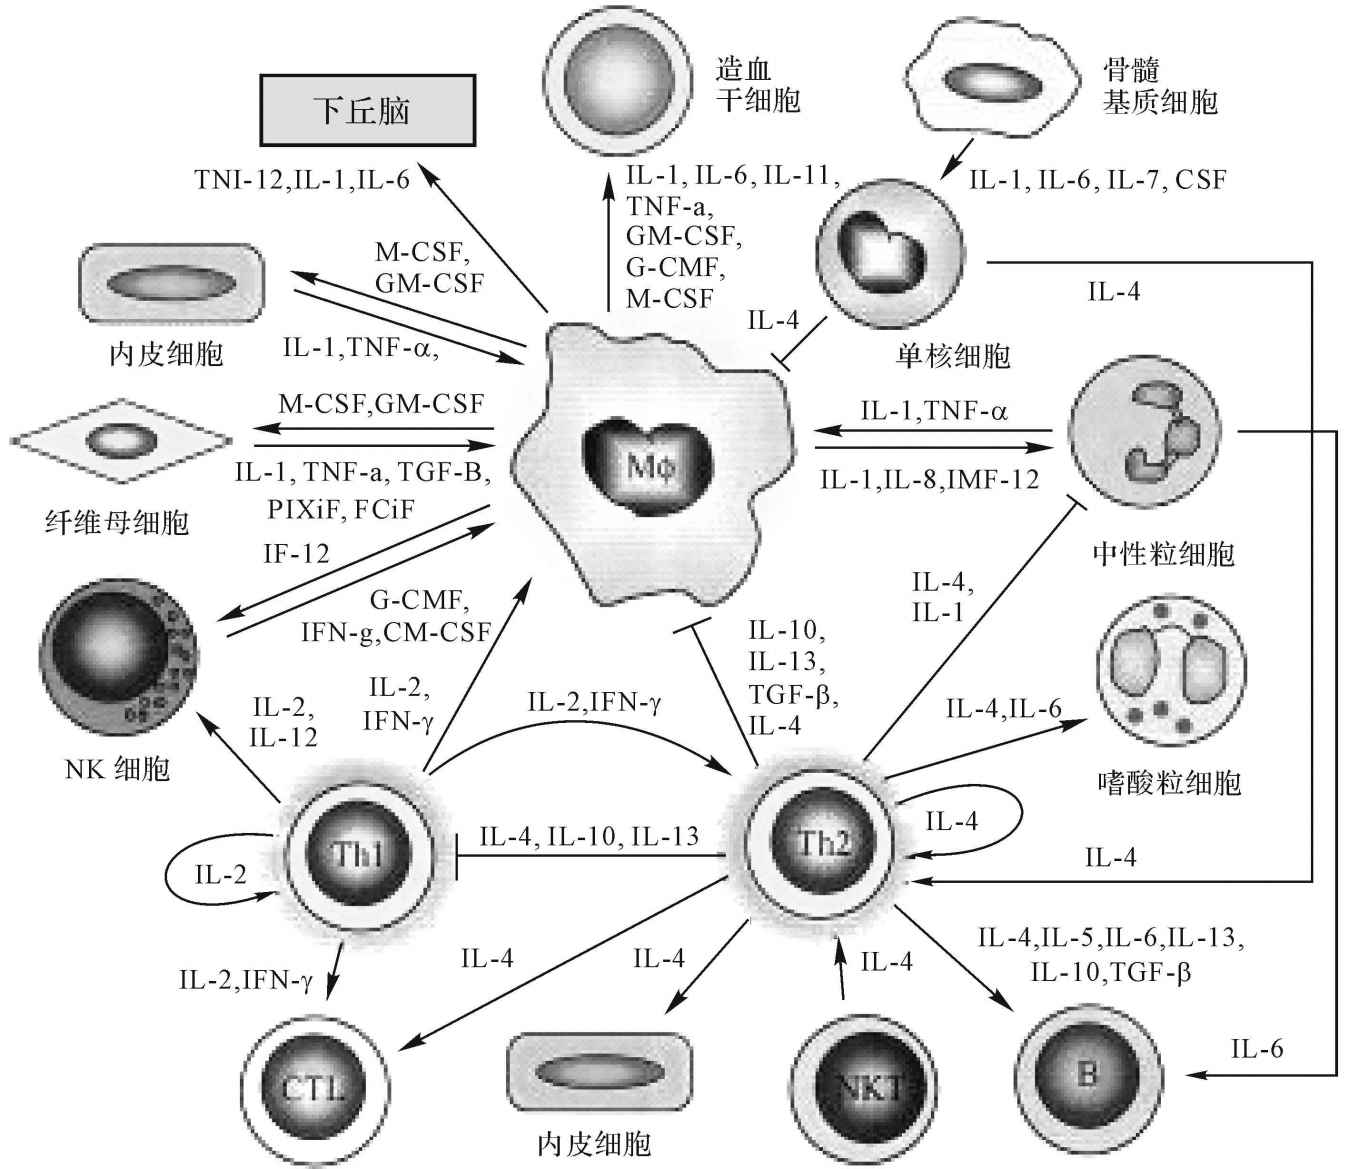
\includegraphics[width=.6\textwidth]{./images/Image00093.jpg}
 \captionsetup{justification=centering}
 \caption{细胞因子的网络性}
 \label{fig6-3}
  \end{figure} 

5.细胞因子作用具有两面性。

(1)生理条件下:发挥免疫调节,抗感染、抗肿瘤。如IL-1局部低浓度参与免疫调节:协同刺激APC和T细胞活化,促进B细胞增殖和分泌抗体。

(2)大量产生引起病理现象。如IL-1大量分泌引起内分泌效应:诱导肝脏急性期,蛋白合成;引起发热和恶病质。

\section{细胞因子种类}

细胞因子的种类繁多,功能各异。其分类可按照细胞因子来源、作用的靶细胞不同或按其主要生物学功能来命名并进行归类。


\subsection{白细胞介素(interleukin,IL)}

\begin{figure}[!htbp]
 \centering
 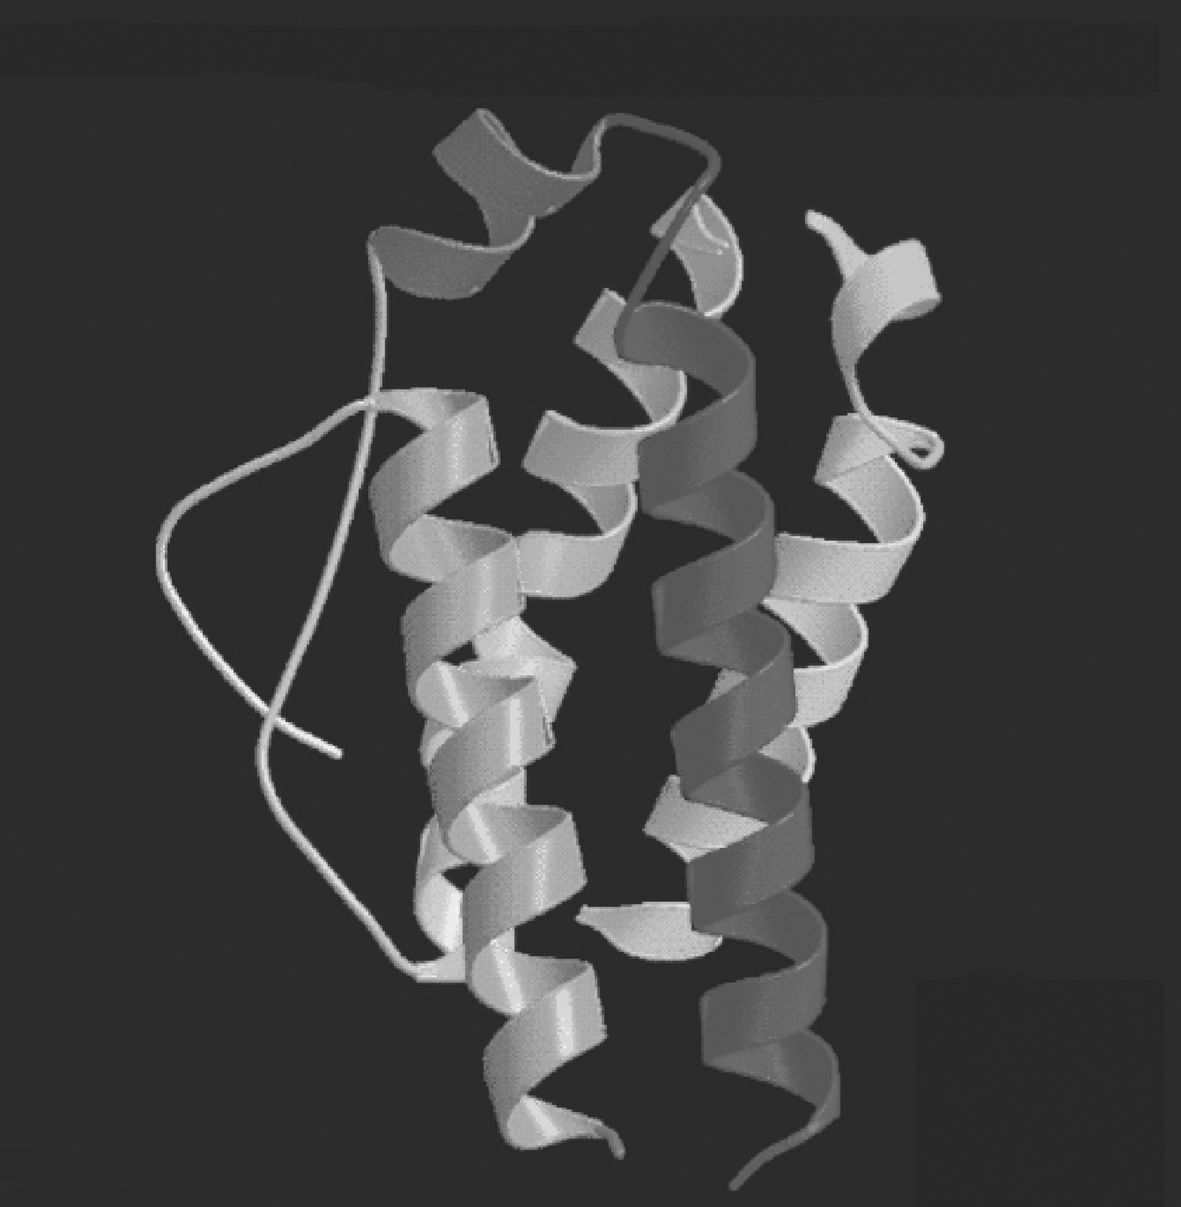
\includegraphics[width=.6\textwidth]{./images/Image00094.jpg}
 \captionsetup{justification=centering}
 \caption{白细胞介素-2}
 \label{fig6-4}
  \end{figure} 

IL是一组由淋巴细胞、单核吞噬细胞和其他免疫细胞产生的能介导白细胞和其他细胞间相互作用的细胞因子,如图\ref{fig6-4}所示。自上世纪80年代起,鉴于陆续发现的多数细胞因子均来源于白细胞,并参与白细胞间的信息交通,故将它们统称为白细胞介素。目前已证实,白细胞以外的其他某些细胞也可产生IL,但仍沿用此命名。IL的主要作用:调节细胞生长、分化,参与免疫应答和介导炎症反应。IL有33种以上:IL1~IL33。


\subsection{干扰素(interferon,IFN)}

IFN具有干扰病毒复制的作用,故得名。现已证实,干扰素具有十分广泛的生物学活性,在免疫应答和免疫调节中发挥重要作用,也是主要的促炎细胞因子之一。

根据干扰素的来源、生物学性质及活性,可将其分为IFN-α、IFN-β和IFN-γ。其中,IFN-α主要由单核/巨噬细胞(及B细胞、成纤维细胞)产生,至少有15个成员;IFN-β主要由成纤维细胞产生。二者又称I型干扰素,主要的生物学活性是抑制病毒复制、抑制多种细胞增殖、参与免疫调节及抗肿瘤等。IFN-γ又称Ⅱ型干扰素,主要由活化的T细胞和NK细胞产生,生物学活性为:抗病毒、抑制细胞增殖、激活巨噬细胞、促进多种细胞表达MHC抗原、促进Th1细胞分化、参与炎症反应等。


\subsection{肿瘤坏死因子(tumor necrosis factor,TNF)}

此因子由于其在体内外均可直接杀伤肿瘤细胞而得名。其家族成员约有30个,其中:TNF-α主要由单核/巨噬细胞及其他多种细胞产生,具有极为广泛的生物学活性,例如:参与免疫应答、抗肿瘤、介导炎症反应、参与内毒素休克、引起恶液质等。

TNF-β又称为淋巴毒素(limphotoxin,LT),主要由淋巴细胞、NK细胞等产生,其生物学活性与TNF-α类似。


\subsection{集落刺激因子(colony stimulating factor,CSF)}

CSF是一组在体内外均可选择性刺激造血祖细胞增殖、分化并形成某一谱系细胞集落的细胞因子,包括巨噬细胞CSF(macrophage-CSF,M-CSF)、粒细胞CSF(granulocyte-CSF,G-CSF)和巨噬细胞/粒细胞CSF(GM-CSF)等。此外,IL-3可刺激多谱系细胞集落形成,又称为multi-CSF;干细胞因子(stem
cell
factor,SCF)可刺激干细胞分化为不同谱系血细胞;红细胞生成素(erythropoietin,EPO)可促进红细胞增生、分化和成熟。上述因子也可视为CSF家族成员。


\subsection{生长因子(growth factor,GF)}

GF乃一类可介导不同类型细胞生长和分化的细胞因子。根据其功能和作用的靶细胞不同,分别命名为转化生长因子β(transforming
growth factor-β,TGF-β)、神经生长因子(nerve growth
factor,NGF)、表皮生长因子(epithelial growth
factor,EGF)、成纤维细胞生长因子(fibroblast growth
factor,FGF)、血小板源生长因子(platelet-derived growth
factor,PDGF)、血管内皮细胞生长因子(vascular endothelial cell growth
factor,VEGF)等。


\subsection{趋化因子(chemokine)}

趋化因子是一类对不同靶细胞具有趋化效应的细胞因子家族,已发现50余个成员。该家族成员依据其分子N端半胱氨酸的数目及其间隔,可分为CC、CXC、C、CX3C四个亚家族。

CXC亚家族(如IL-8)主要对中性粒细胞具有趋化和激活作用(图\ref{fig6-5})。

CC亚家族,如单核细胞趋化蛋白(monocyte chemoattractant
protei,MCP)和RANTES(reduced upon activation normal T expression and
secretion),主要对中性粒细胞以外的白细胞,尤其是单核/巨噬细胞具有趋化和激活作用。

\begin{figure}[!htbp]
 \centering
 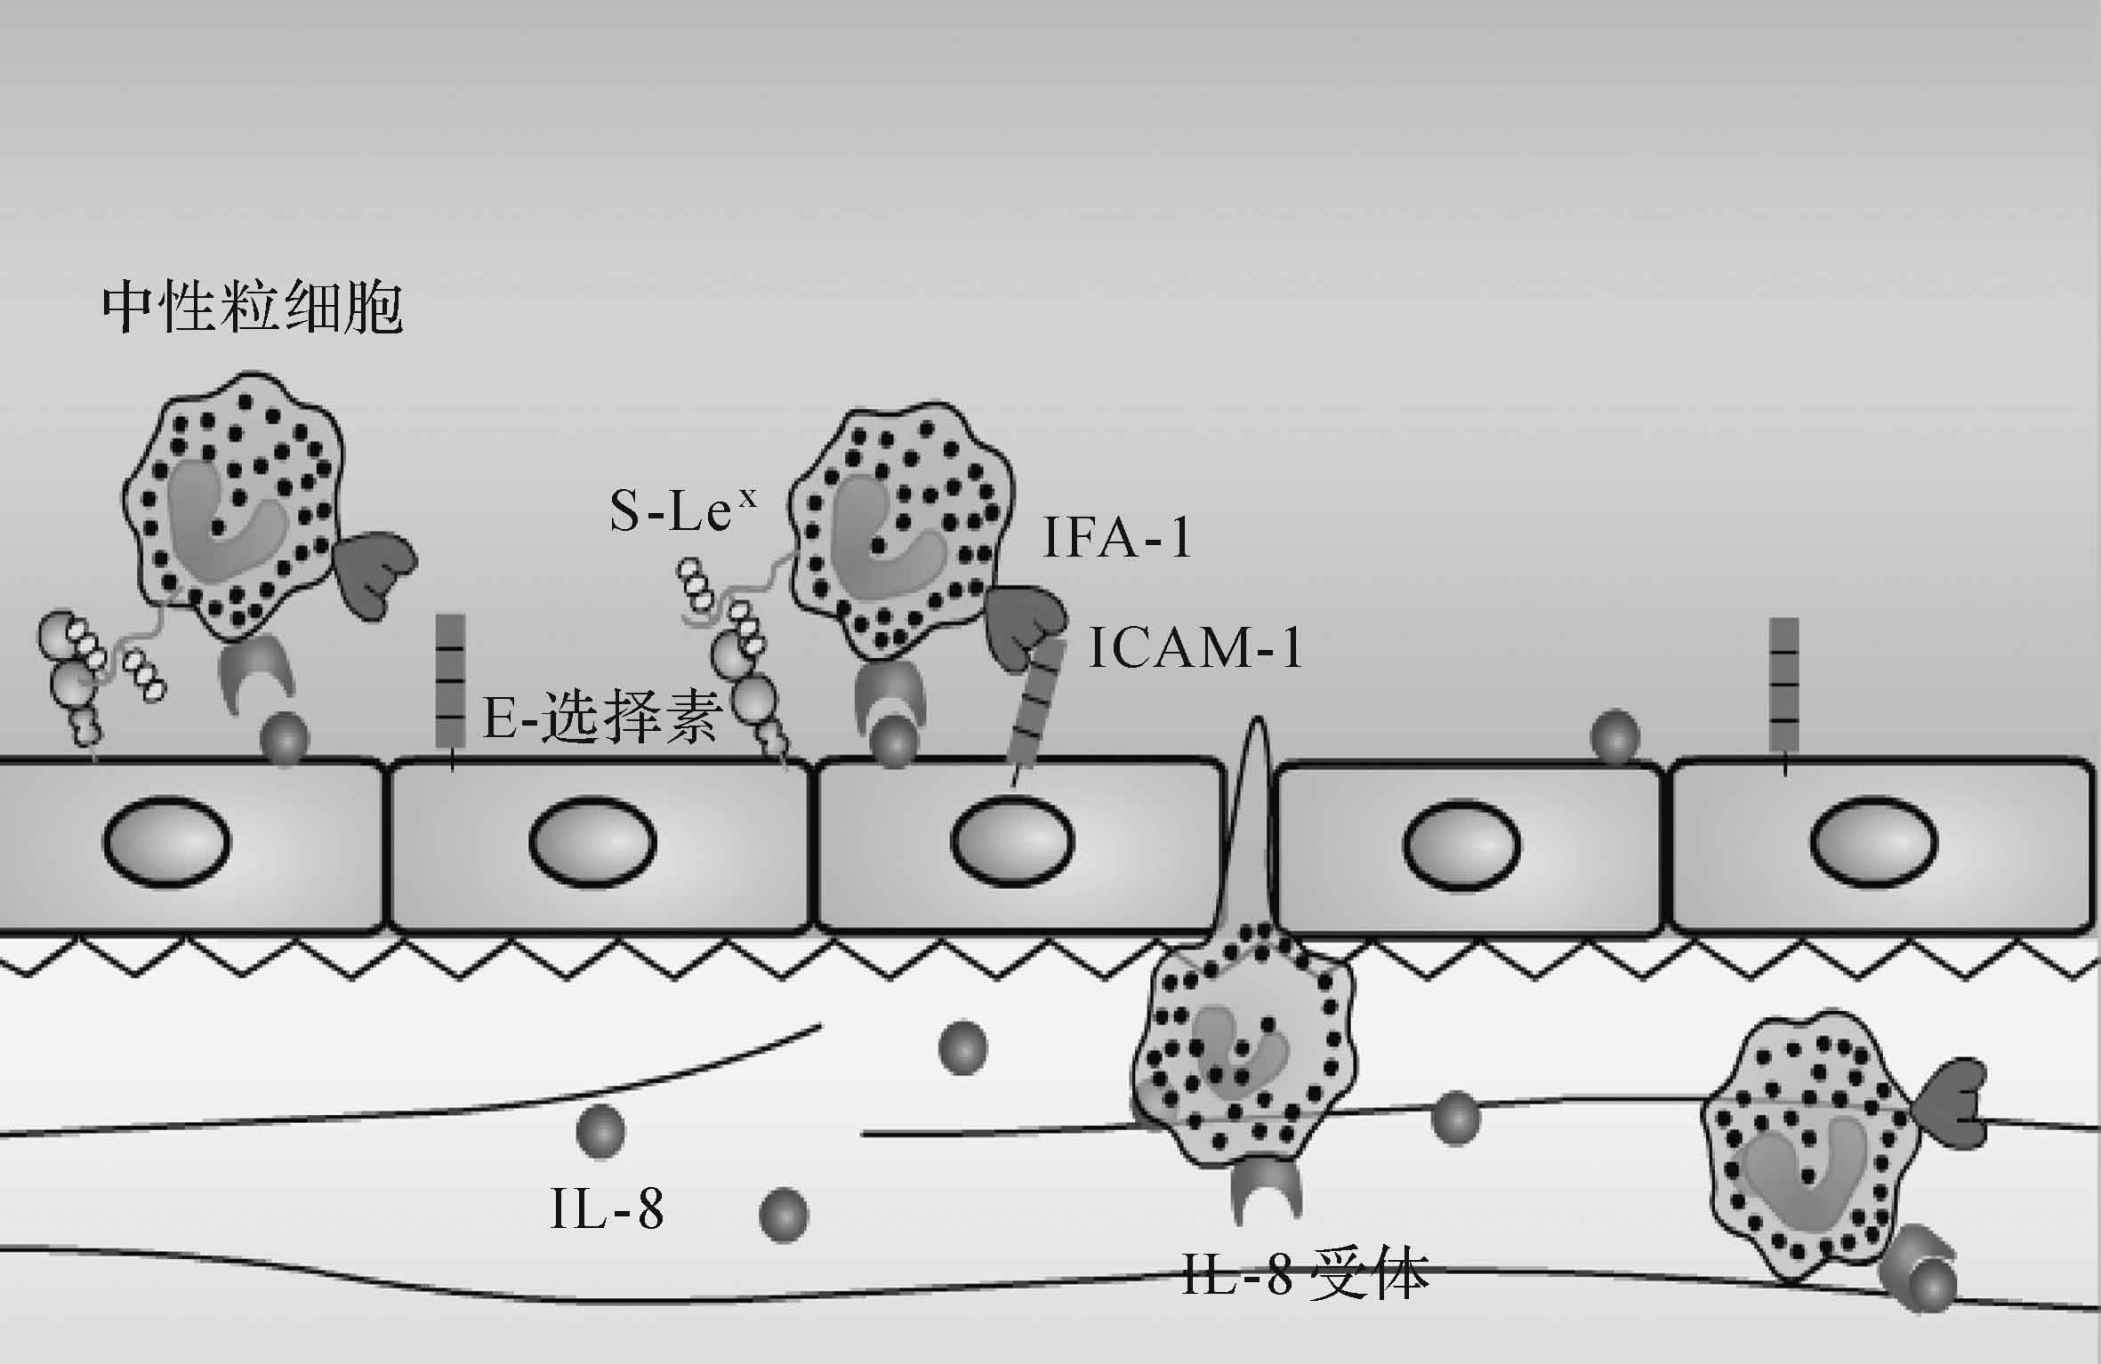
\includegraphics{./images/Image00095.jpg}
 \captionsetup{justification=centering}
 \caption{对中性粒细胞的趋化作用}
 \label{fig6-5}
  \end{figure} 

\section{细胞因子的生物学活性}

细胞因子的生物学活性如图\ref{fig6-6}所示。

\begin{figure}[!htbp]
 \centering
 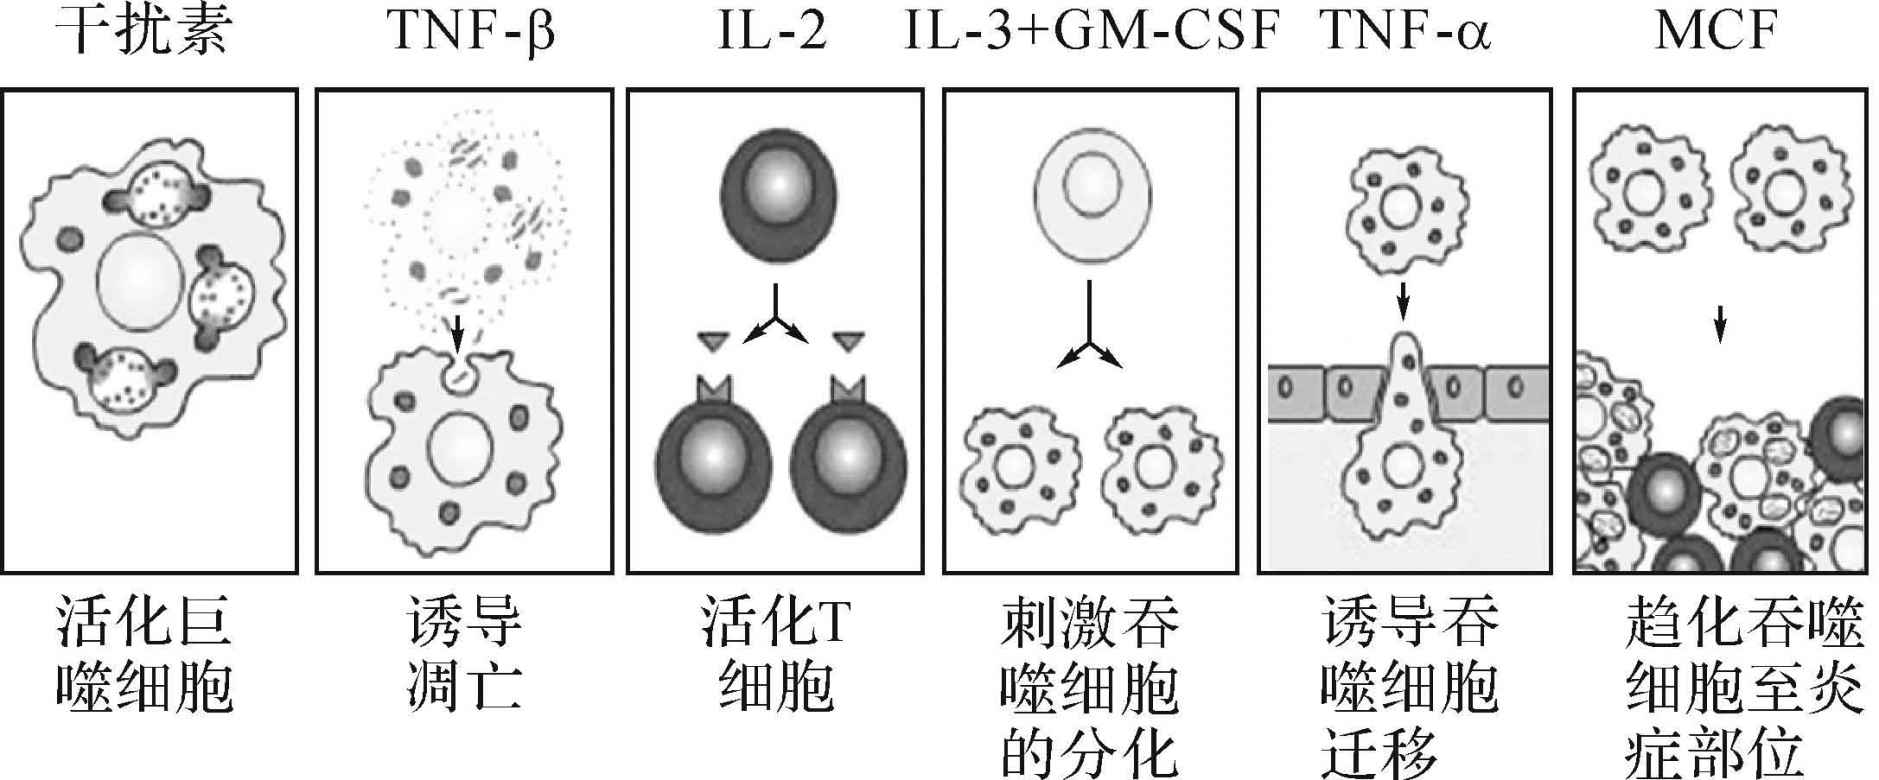
\includegraphics{./images/Image00096.jpg}
 \captionsetup{justification=centering}
 \caption{细胞因子的生物学活性}
 \label{fig6-6}
  \end{figure} 


\subsection{介导和调节固有免疫}

介导固有免疫的细胞因子主要由单核-巨噬细胞分泌,具有抗病毒、抗细菌感染的作用。

(一)抗病毒

I型干扰素(IFN-α/β)、IL-15和IL-12是三种重要的抗病毒细胞因子(图\ref{fig6-7})。受到病毒感染的细胞可合成和分泌IFN-α/β,刺激邻近的细胞合成抑制RNA及DNA病毒复制的酶类使其进入抗病毒状态。

IFN-α/β:具有增强NK细胞裂解病毒感染细胞的功能,增强CTL的活性。

IL-12:能增强激活的NK细胞和CD8\textsuperscript{+} T细胞裂解靶细胞。

IL-15:能刺激NK细胞的增殖。抗病毒细胞因子的这些功能均有利于消除病毒的感染。

\begin{figure}[!htbp]
 \centering
 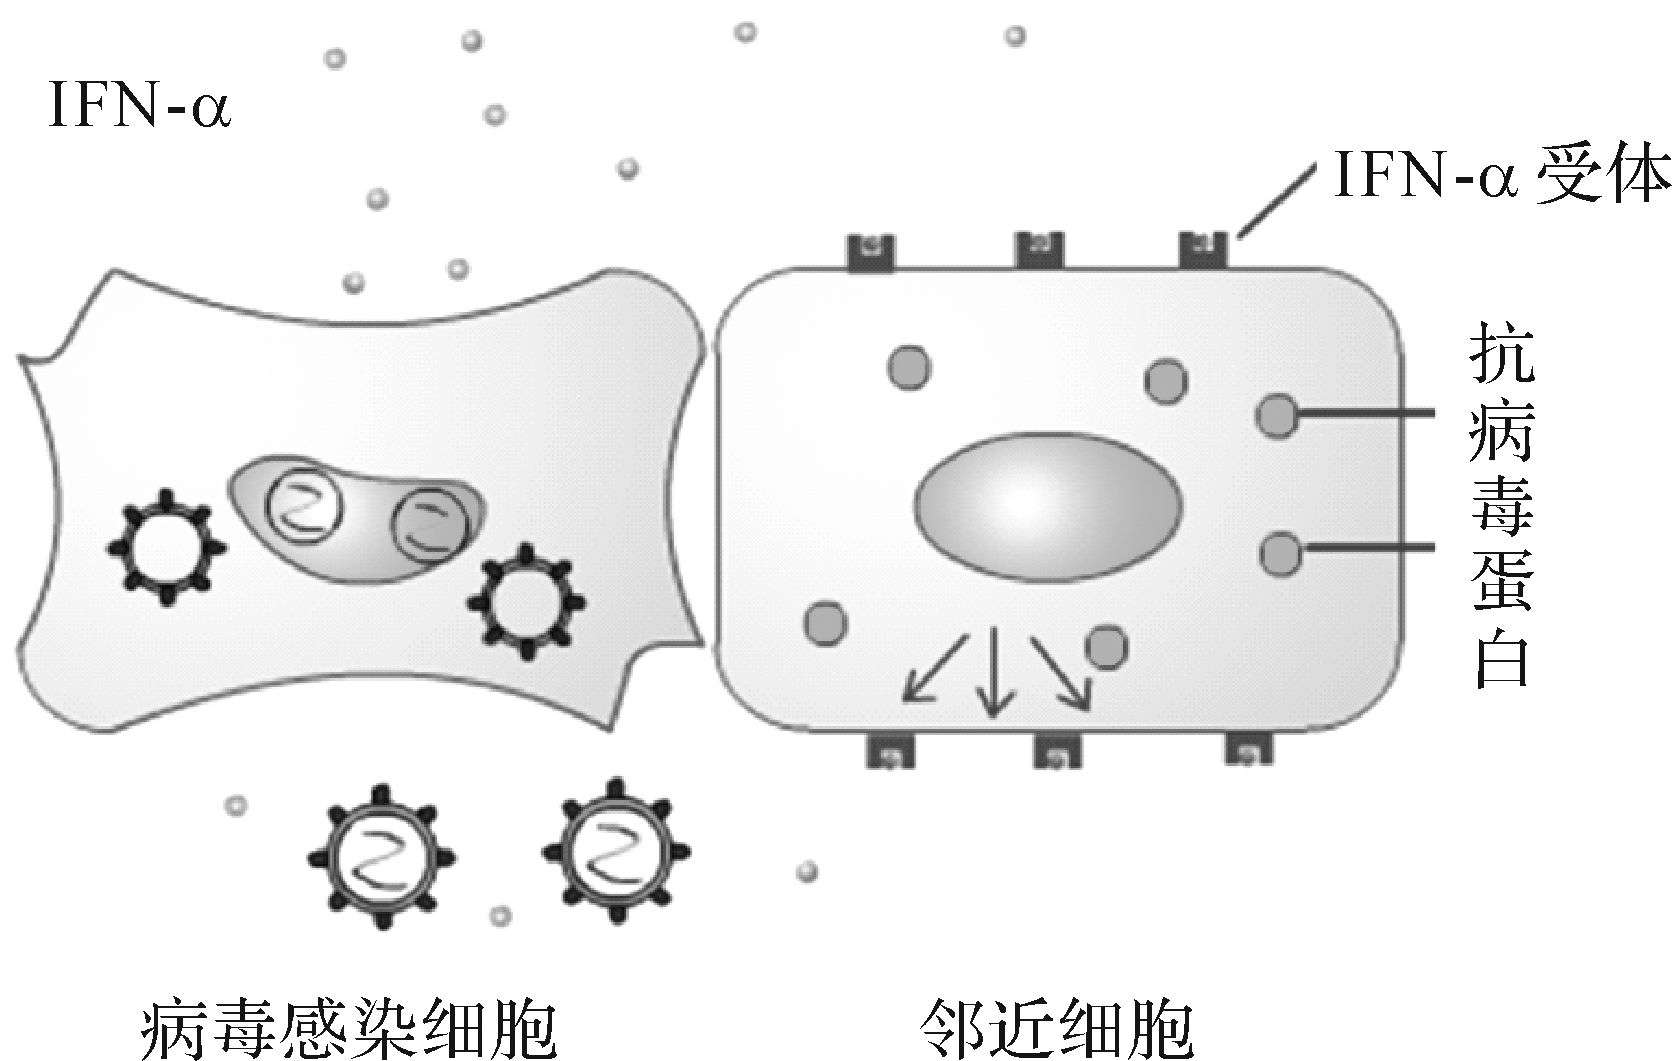
\includegraphics{./images/Image00097.jpg}
 \captionsetup{justification=centering}
 \caption{干扰素的抗病毒作用}
 \label{fig6-7}
  \end{figure} 

(二)抗细菌感染

TNF、IL-1、IL-6和趋化性细胞因子被称为促炎症细胞因子,是启动抗菌炎症反应的关键细胞因子,可促进肝脏产生急性期蛋白(acute
phage
protein),增强机体抵御致病微生物的侵袭;还是内源性致热原,可作用于体温调节中枢,引起发热。

TNF的作用:(1)
引起白细胞在炎症部位的聚集,(2)激活炎性白细胞去杀灭微生物。

IL-1的作用:刺激单个核吞噬细胞和内皮细胞分泌趋化性细胞因子。

IL-6的作用:刺激肝细胞分泌急性期蛋白,有利于抑制和排除细菌(图\ref{fig6-8})。

\begin{figure}[!htbp]
 \centering
 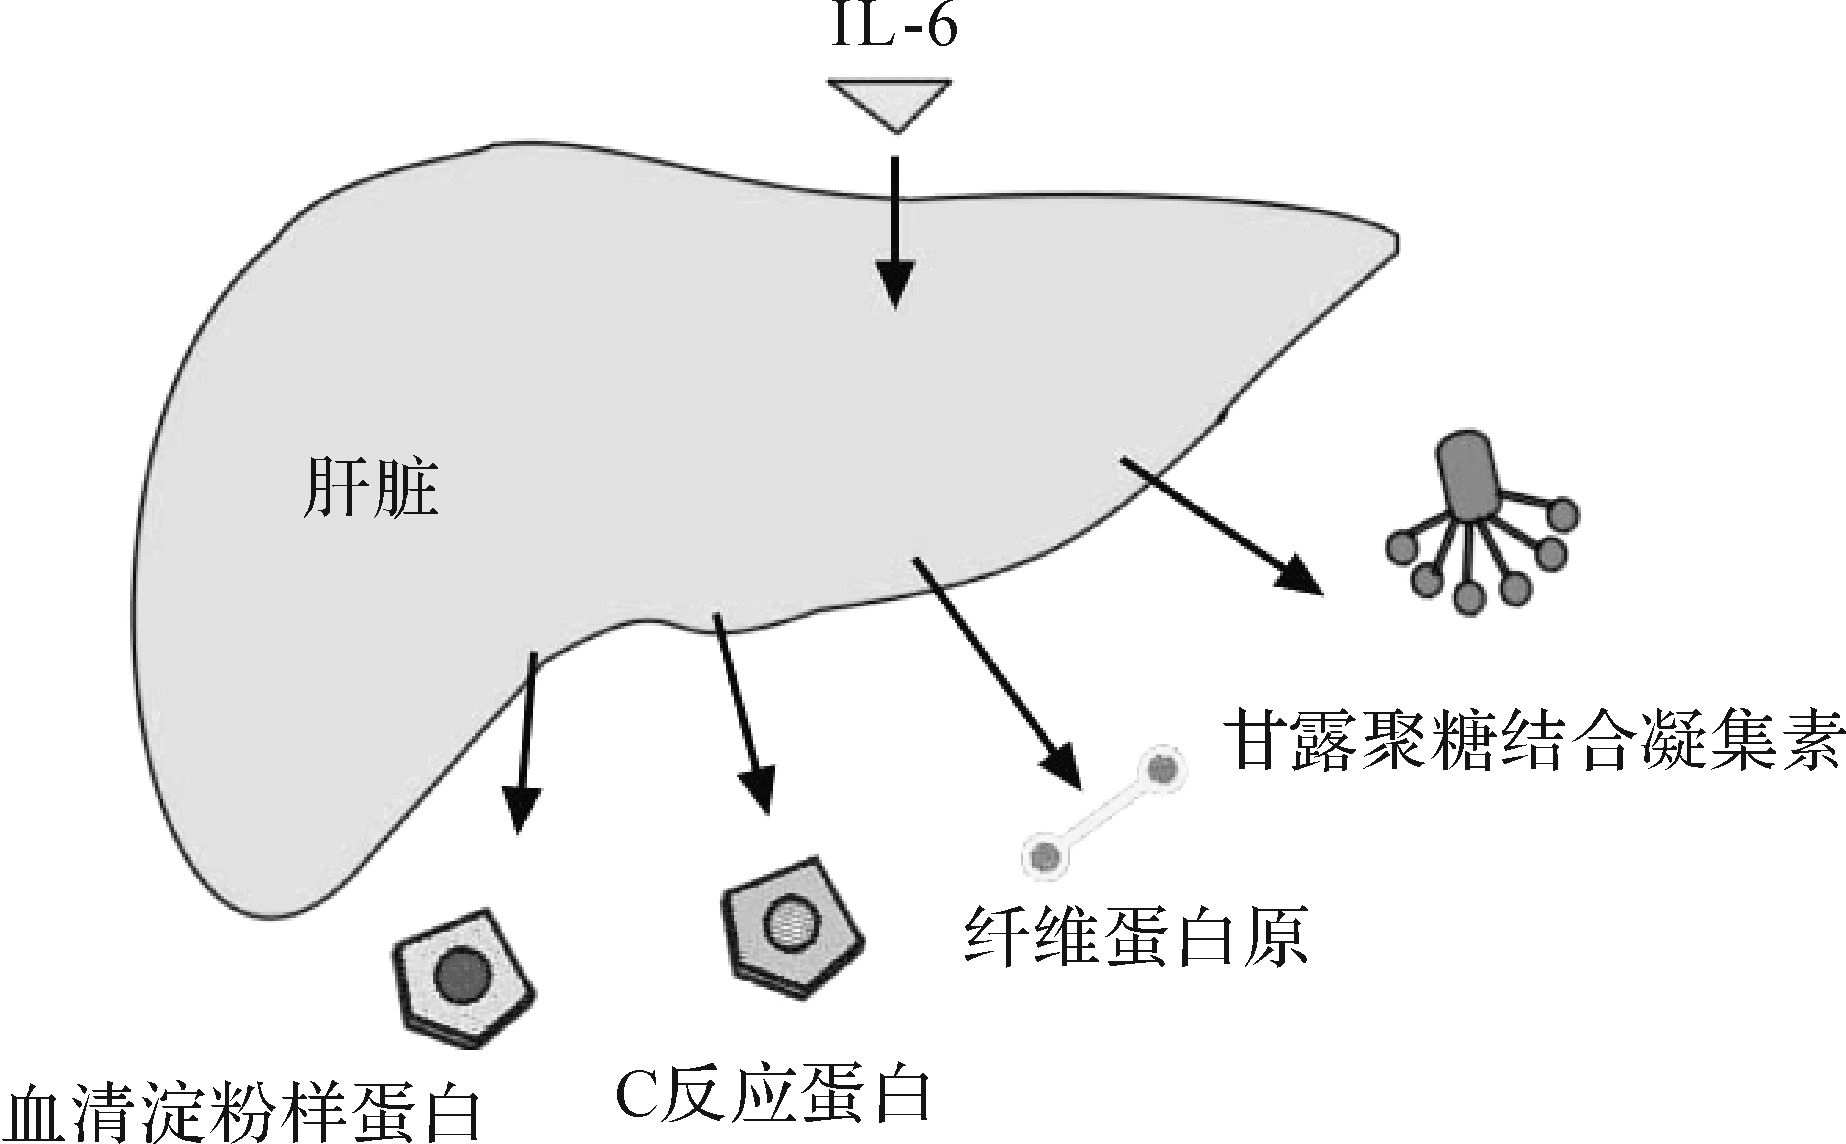
\includegraphics{./images/Image00098.jpg}
 \captionsetup{justification=centering}
 \caption{细胞因子诱导急性期蛋白的合成}
 \label{fig6-8}
  \end{figure} 


\subsection{介导和调节特异性免疫应答}

特异性免疫应答主要由抗原活化的T淋巴细胞分泌,调节淋巴细胞的激活、生长、分化和发挥效应。在受到抗原的刺激后,淋巴细胞的活化受到细胞因子的正负调节(图\ref{fig6-9})。如:IFN-γ通过刺激抗原递呈细胞表达MHC-Ⅱ类分子促进CD\textsuperscript{+}
\textsubscript{4}
T细胞的活化;IL-2、IL-4、IL-5、IL-6等可促进T/B细胞激活、增殖和分化;趋化因子可诱导不同免疫细胞的定向运动,并参与其激活;TNF等参与免疫效应阶段的细胞毒作用;TGF-β可抑制巨噬细胞的激活。

\begin{figure}[!htbp]
 \centering
 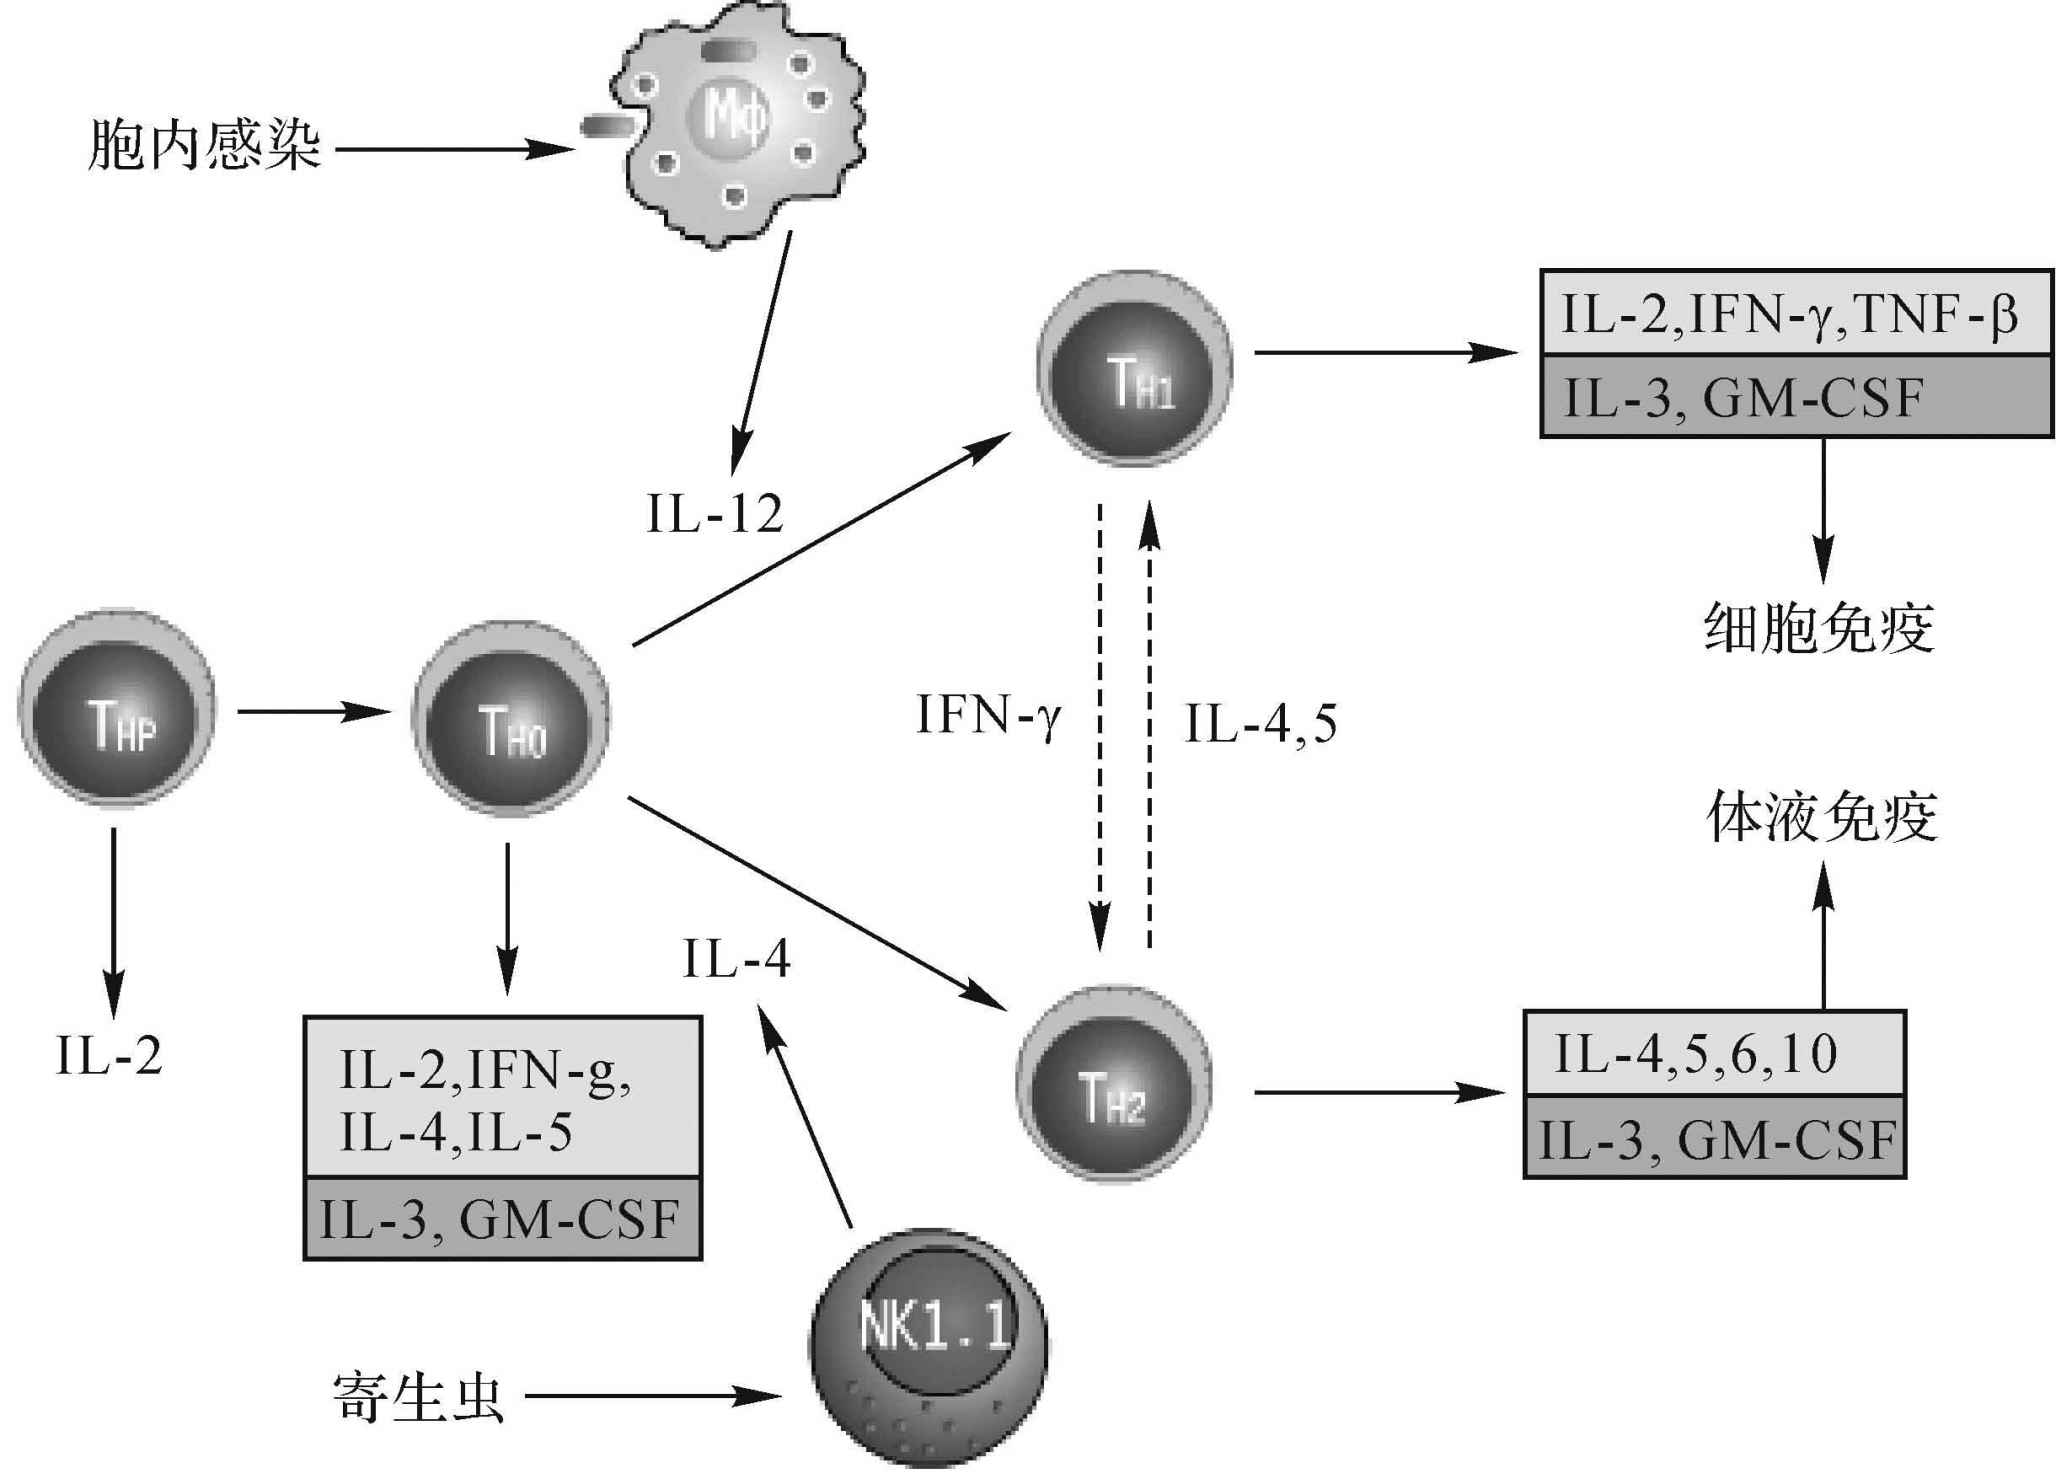
\includegraphics{./images/Image00099.jpg}
 \captionsetup{justification=centering}
 \caption{细胞因子对Th1和Th2细胞分化的调节作用}
 \label{fig6-9}
  \end{figure} 


\subsection{刺激造血}

由骨髓基质细胞和 T
细胞等产生刺激造血的细胞因子在血细胞的生成方面起重要作用,其生成过程如图\ref{fig6-10}所示。

\begin{figure}[!htbp]
 \centering
 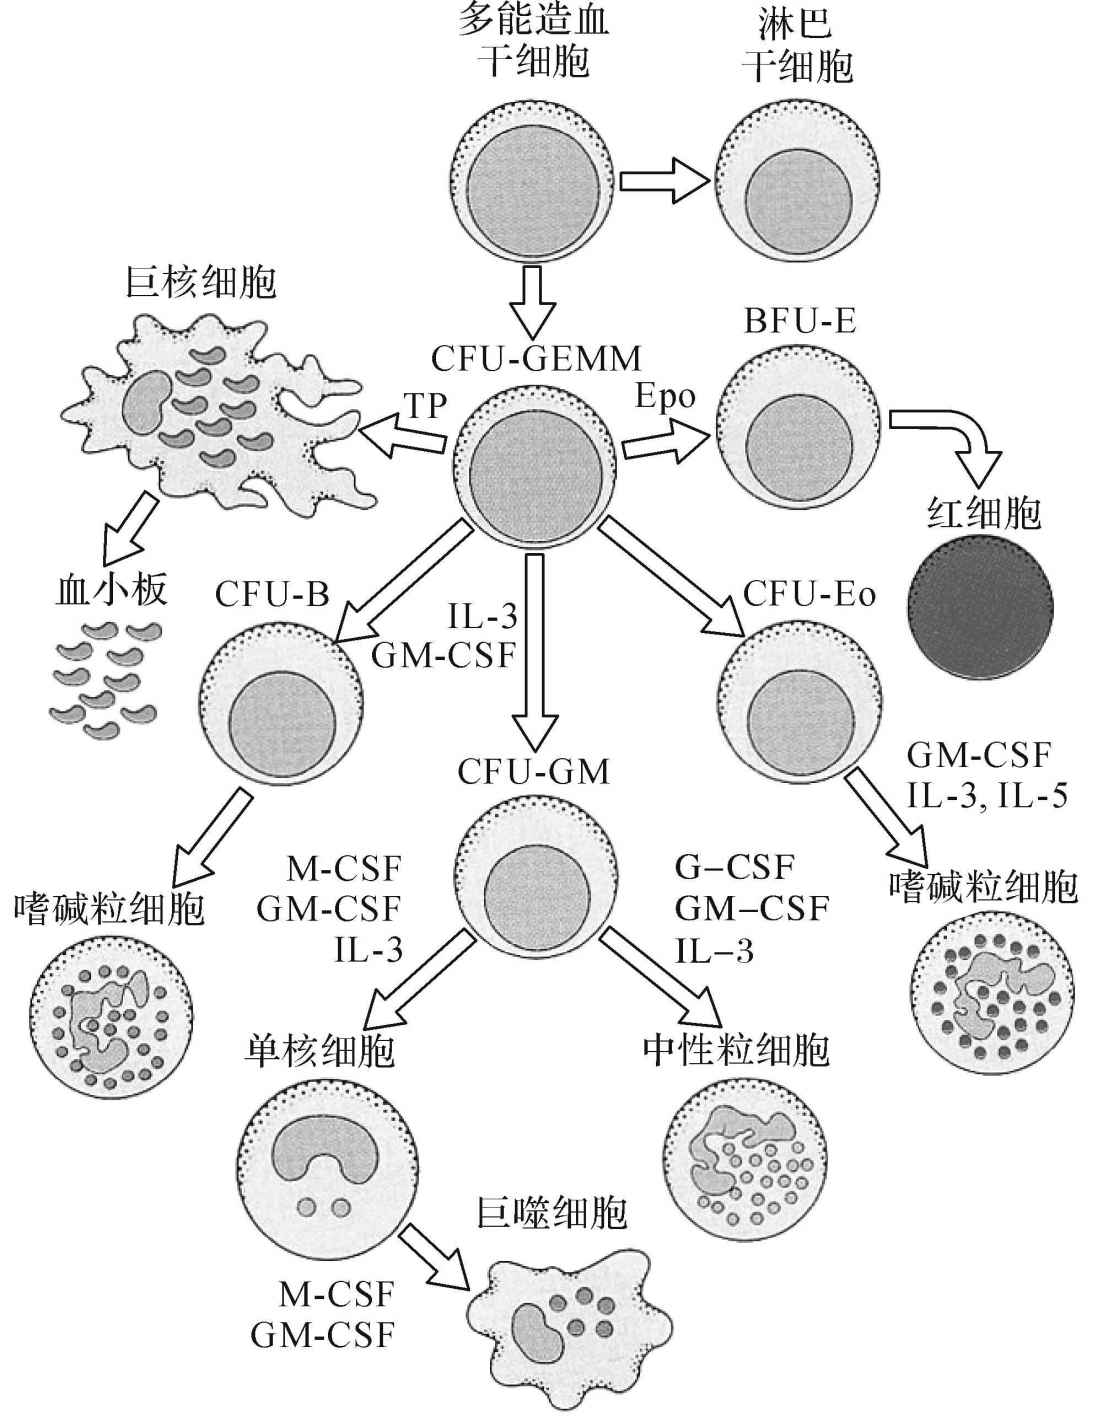
\includegraphics[width=.5\textwidth]{./images/Image00100.jpg}
 \captionsetup{justification=centering}
 \caption{细胞因子刺激血细胞生成}
 \label{fig6-10}
  \end{figure} 

\section{重组细胞因子类药物}

目前国内市场上主要的国产重组细胞因子类药物包括IFN、IL-2、G-CSF、重组表皮生长因子(rEGF)、重组链激酶(rSK)等15种基因工程药物。组织溶纤原激活剂(T-PA)、IL3、重组人胰岛素、尿激酶等十几种多肽药物正处于临床Ⅱ期试验阶段,单克隆抗体的研制已从实验阶段进入临床阶段。正在开发研究中的项目包括采用新的高效表达系统生产重组凝乳酶等40多种基因工程新药。

在欧美市场上,对现有重组药物进行分子改造而开发的某些第二代基因药物已经上市,如重组新钠素、胞内多肽等。另外,重组细胞因子融合蛋白、人源单克隆抗体、反义核酸,以及基因治疗、新的抗原制备技术、转基因动物生产等,均取得了实质性的进展。国外生物医药的目前发展动向,主要反映在以下几方面。


\subsection{与血管发生有关的细胞因子}

肿瘤血管生长因子(tumor angiogenesis
factors,TAF)包括研究较多的血管内皮生长因子(vascular endothelial
growth factor,VEGF)、成纤维细胞生长因子(fibroblast growth
factor,FGF)、血小板源生长因子(platelet-derived growth
factor,PDGF)等,它们促进肿瘤新生微血管的生长。临床研究表明,阻断VEGF受体2(VEGFR-2)和PDGF受体β(PDGFR-β)等,可达到通过抗血管生成来治疗肿瘤的目的。1998年,美国科研人员发现两种用于治疗癌症的血管发生抑制因子(即抗血管生长因子)和内皮抑制素,以及一种抗血管生长蛋白,即血管抑制素(vasculostatin),都有较好的疗效。另外,VEGF、FGF和血管生长素(angiopoietin)等能够通过刺激动脉内壁的内皮细胞生长来促进形成新的血管,从而对冠状动脉疾病和局部缺血产生治疗作用。


\subsection{集落刺激因子(CSF)}

CSF有四种:GM-CSF、G-CSF、M-CSF和Multi-CSF,它们对造血细胞的生长分化起介导作用。在临床上,重组CSF能提高病人的耐受力,增加化疗强度和敏感性,加速骨髓移植后造血功能的恢复,因此已用于治疗肿瘤放疗和化疗后的白细胞减少、再生障碍性贫血、白血病和粒细胞缺乏症等。因CSF能增强抗原递呈细胞的免疫功能,故可利用重组人CSF基因的反转录病毒载体,转导鼠和人肿瘤细胞,通过这样的途径制作肿瘤疫苗,诱导机体产生有效的抗肿瘤免疫反应。重组CSF还被广泛用作疫苗佐剂,协助接种疫苗。但在副作用方面,重组CSF可引起轻微的发烧、寒战、恶心、呕吐、无力、头痛、肌痛和关节痛等。


\subsection{干细胞因子(SCF)}

SCF有多种重要的生理功能,是一种主要对造血细胞起重大作用的细胞因子,在自体外周血造血前体细胞的移植、放疗和化疗的辅助治疗、再生障碍性贫血等血液病的治疗及遗传性骨髓缺陷综合征的治疗方面,有良好的应用前景。在临床上,SCF可用于建立体外造血前体细胞库,如骨髓库、脐血库,并进行体外扩增。SCF对肿瘤免疫治疗中树突状细胞的扩增、基因治疗中靶细胞的扩大等也具有价值。1998年,曹诚等在大肠杆菌中高效表达了可溶形式的人SCFA,目的蛋白质占菌体总蛋白质的40%左右。表达产物复性后,经离子交换、凝胶过滤层析后测定,重组人SCF的氨基端序列及其他理化性质与天然人SCF相同,可刺激人骨髓细胞增殖,导致粒细胞-巨噬细胞集落(CFU-GM)明显增加,显示出天然SCF的生物功能活性。


\subsection{肿瘤坏死因子(TNF)}

TNF是人体内对肿瘤有直接杀伤作用的一种细胞因子,可使瘤体缩小或消失,对多种肿瘤的中晚期患者有一定治疗作用,但在临床应用中发现有明显的毒副反应,如发热、寒战、恶心呕吐、头痛、肝肾功能改变等。20世纪80年代,许多国际机构因没有很好地解决毒副作用问题而放弃了有关重组人TNF的研制。近年来,第二军医大学在国际上首创二轮基因扩增引物法,通过哺乳动物细胞的表达,成功地获得重组人TNF。它能选择性地杀死癌细胞,毒性低、疗效高,目前已完成前期临床试验,即将作为国家一类新药广泛应用于临床。


\subsection{白细胞介素(IL)}

IL是一组介导白细胞间相互作用的细胞因子,在免疫系统中发挥重要的生理功能。自1979年第一个IL被命名后,新的IL相继被发现和克隆。近期的发现均借助计算机克隆技术,即利用商业化的EST数据库,在同源性分析的基础上进行基因克隆、细胞表达和功能分析,最终确认新的IL。这条技术路线实质上是从基因到蛋白质再到体内外功能的路线。

五个新的正式排序的IL包括IL-19、IL-20、IL-21、IL-22和IL-23。它们目前虽未见诸临床报道,但均具备可观的药物开发前景。1999年,美国HGS公司报道了IL-19。它主要在活化的单核巨噬细胞中表达,对于抗原递呈细胞具有调节和促增殖的效应。2000年6月,美国HGS公司报道了IL-20及其受体。IL-20主要表达于脊髓、睾丸和小肠中。将重组IL-20注射入小鼠的腹腔,可明显刺激中性粒细胞的移动。2000年11月,ZymoGenetics公司发现含信号肽和跨膜区的IL-21受体。IL-21能促进骨髓NK细胞的增殖和分化,与抗CD40抗体协同刺激B细胞的增殖,与抗CD3抗体协同刺激T细胞的增殖。2000年10月,Genentech公司通过检索和测试发现IL-22,它能活化多种细胞系的STAT1、STAT3和STAT5,主要表达于活化的T细胞中。该公司还通过细胞转染实验发现IL-22受体。2000年11月,DNAX研究所发现IL-23。这种分子能促使活化的T细胞增殖并产生γ干扰素,还可诱导记忆性T细胞增殖。


\subsection{促红细胞生成素(EPO)}

人EPO是一种高度糖基化的蛋白质类激素样物质,主要来自肾脏,极小部分来自肝脏,能促进红细胞的生成。在临床上,EPO主要用于治疗各种贫血,对慢性肾衰性贫血起补充治疗作用,对于诸如类风湿引起的贫血也有较好的疗效。天然存在的EPO药源极为匮乏,必须从贫血病人的尿中提取,不能满足医疗需求。1985年,国外研究者成功地从胎儿肝中克隆出EPO基因,通过基因工程手段大量生产重组EPO由此成为可能。


\subsection{血小板生成素(thrombopoietin,TPO)}

TPO是一种作用于巨核细胞-血小板生成系统的造血细胞生长因子,能特异地刺激巨核细胞增殖、分化、成熟和产生血小板,从而增加血循环中的血小板数量。在临床上,TPO对血小板减少症有良好疗效,属特效药物。2003年8月,重组人TPO由沈阳三生药业完成Ⅱ、Ⅲ期临床试验,是迄今研制成功的第三个具有自主专利权的国家一类新药。复旦大学中山医院等的临床试验结果表明,该药适用于预防和治疗肿瘤化疗引起的血小板减少及原发性血小板减少症,填补了骨髓三大血细胞系中缺乏调节巨核细胞特异性药物的空白。但该药存在免疫原性强、制备成本高的缺点,仍有待改进。


\subsection{白血病抑制因子(LIF)}

LIF是一类高度糖基化的多肽细胞因子,能抑制胚胎干细胞的体外分化,维持其传代和多能性。20世纪60年代末,曾发现一种诱导小鼠M1白血病细胞系分化为正常细胞的分化诱导因子。此因子能促进白血病M1细胞的分化,并抑制其增殖,所以被命名为白血病抑制因子(leukemia
inhibitory
factor,LIF)。在临床上,LIF与子宫内着床、急性期反应等许多过程及征象密切相关,还可抑制脂蛋白脂酶的活性,促进钙吸收,使血小板增加,刺激肝细胞合成急性反应蛋白,并参与胚胎及造血系统的发育,还能促进神经肌肉的生长并维持垂体的功能。1999年,我国研究者根据人LIF基因的cDNA序列,通过合理的引物设计、链延伸反应、PCR反应和分子克隆等步骤,成功地合成了编码成熟LIF蛋白的基因片段,并将其克隆至pUC18载体质粒上。这一成果有助于重组LIF药物的开发。


\subsection{转化生长因子(TGF)}

TGF主要由肿瘤细胞产生,是一种小肽分子,包括目前已发现的α、β等五种亚型。

TGF-α为分泌性蛋白质,在血液和尿液中均能检测到。它通过与细胞的表皮生长因子受体(EGFR)结合而实现其生理作用,以自分泌和旁分泌的形式参与调节细胞的增殖和分化。在正常组织中一般难以检测到TGF-α,但在许多肿瘤和肿瘤细胞株里却有TGF-α的过量合成。因此,TGF-α在肿瘤的诊断和预后、临床外伤的治疗等许多方面有应用价值。

TGF-β是一类具备激素样活性的多肽生长因子,可刺激细胞的增殖和分化,对细胞进行双向调节。在临床应用方面,宾夕法尼亚大学的研究者研制出抗TGF-β抗体,能治疗糖尿病性肾病。此病的患者均有TGF-β过度表达的征象,采用抗TGF-β的中和抗体,可明显改善肾脏的结构与功能。另外还发现,TGF-β在肿瘤治疗中能刺激并抑制新生血管的形成。我国研究者于2001年研究了在鼠肠黏膜不同状态下的TGF表达水平,发现TGF-β与肿瘤密切相关。

\noindent\textbf{【理解与思考】}

1.综合机体的生理过程,你能表述细胞因子的作用吗?

2.细胞因子在炎症中,是如何起作用的?

\noindent\textbf{【课外拓展】}

1.细胞因子受体分类、特点。

2.细胞因子的抑制性调节因素有哪些?

3.细胞因子的效应机制如何?

4.细胞因子产生的调节机理如何?

5.重组细胞因子生产的主要工艺是什么?

\noindent\textbf{【课程实验与研究】}

1.如何检测某种细胞因子的生物活性?

2.请设计一种方案,检测免疫细胞能释放哪些细胞因子。

3.请设计检测肿瘤坏死因子的医药效果的技术路线。

4.体育项目兴奋剂检测项目有哪些?如何去检测尿样中的细胞因子?

\noindent\textbf{【课程研讨】}

1.以某种细胞因子为例,查阅资料阐述其最新的研究进展与应用前景。

2.细胞因子的产业前景如何?

3.请从正反两方面来阐述每种细胞因子在机体中的作用。

4.目前细胞因子在临床医学上的应用前景如何?

5.你认为机体中可能还有哪些待发现的细胞因子?你的依据是什么?

6.细胞因子产业化的主要瓶颈是什么?破解的途径是什么?

\noindent\textbf{【课后思考】}

1.细胞因子的概念,有哪些特性?

2.细胞因子分为哪些种类?其生物学活性有哪些?

\noindent\textbf{【课外阅读】}

\begin{center}
    \textbf{\Large 肿瘤坏死因子的研究进展与应用前景}
\end{center}

1975年,Carswell等发现接种BCG的小鼠注射LPS后,血清中含有一种能杀伤某些肿瘤细胞或使体内肿瘤组织发生血坏死的因子,称为肿瘤坏死因子。1985年,Shalaby把巨噬细胞产生的TNF命名为TNF-α,把T淋巴细胞产生的淋巴毒素命名为TNF-β。TNF-α由细菌脂多糖活化的单核-巨噬细胞产生,可引起肿瘤组织出血坏死,也称恶病质素;TNF-β由抗原或丝裂原刺激的淋巴细胞产生,具有肿瘤杀伤及免疫调节功能,又称淋巴毒素。尽管两型TNF有不同的细胞来源,DNA水平上也仅有28%的核苷酸序列同源,但两者结合于相同的膜受体,并且具有非常相似的生物学功能。

人TNF-α和TNF-β的基因均位于第6号染色体。成熟TNF-α的分子量约为17kD,而TNF-β略呈异质性,为2025kD。TNF受体存在于几乎所有的有核细胞表面,目前已发现两种TNF受体(TNFRI和TNFRII)。TNFRII的亲和力比较强,TNFRI的亲和力相对弱一些。两者与TNF结合后产生的效应有所不同,TNFRI主要增强细胞毒细胞的活性和促进成纤维细胞生长,而TNFRII主要是增进T细胞增殖。

最初对TNF功能的认识仅限于对肿瘤的特异性杀伤作用,后来发现TNF也具有免疫调节作用,而且参与某些炎症反应的过程。TNF的生物活性与IL-1十分相似,只是TNF的毒性较大,更易引起血管阻塞,抗肿瘤作用更强。低浓度的TNF-α主要在局部发挥作用,高浓度的TNF-α可以进入血流,引起全身性反应。近来的研究表明,人和小鼠TNF-α和TNF-β的基因都与MHC基因紧密连锁,暗示其可能参与免疫调节基因的表达调控。

TNF在体内、体外均能杀死某些肿瘤细胞,或抑制增殖作用。肿瘤细胞株对TNF-α敏感性有很大的差异,TNF-α对极少数肿瘤细胞甚至有刺激作用。用放线菌素D、丝裂霉素C、放线菌酮等处理肿瘤细胞(如小鼠成纤维细胞株L929)可明显增强TNF-α杀伤肿瘤细胞活性。体内肿瘤对TNF-α的反应也有很大的差异,与其体外细胞株对TNF-α的敏感性并不平行。同一细胞系可能有敏感株和抵抗株如L929-S和L929-R。此外,靶细胞内源性TNF的表达可能会使细胞抵抗外源性TNF的细胞毒作用,因此,通过诱导或抑制内源性TNF的表达可改变细胞对外源性TNF的敏感性。巨噬细胞膜结合型TNF可能参与对靶细胞的杀伤作用。

TNF杀伤肿瘤的机理还不十分清楚,与补体或穿孔素杀伤细胞相比,TNF杀伤细胞没有穿孔现象,而且杀伤过程相对比较缓慢。

由于TNF的抗肿瘤作用和多种免疫调节功能,TNF疗法的临床研究已在许多国家开展。动物实验和临床实验均表明,TNF对某些肿瘤具有明显的抑制作用;但是由于副作用较大,为TNF的临床应用造成困难。TNF的副作用包括发热、头痛、恶心、呕吐、全身倦怠、肌肉酸痛等;高剂量时可导致休克、肾功能不全和DIC形成等。建立合理的用药方案及治疗措施,可望降低用量,减轻副作用,达到最佳治疗效果。

静脉注射rhTNF可使部分肿瘤缩小,但是副作用大,人体很难耐受。瘤内注射可在局部出现坏死,且副作用较轻,对某些肿瘤的治疗效果优于静脉注射。已报告的有效病例包括肾癌、胃癌、肝癌等,并使转移性大肠癌腹水减少。鉴于TNF可直接杀伤瘤细胞而不太损伤正常细胞,比化疗药物毒性小,rhTNF可望较其他细胞因子更快地大量应用于临床。

根据以上综述,在临床上单独使用TNF用量大,不容易获得好的效果,患者常因不能耐受其副作用而中止用药。将其他具有肿瘤抑制作用的细胞因子(如IL-2、IFN等)或某些抗肿瘤药物与TNF联合应用,既可减少各种药物的用量、降低毒副作用,又可提高疗效,不失为肿瘤治疗的一种可行方法。此外,由于TNF对肺癌的杀伤能力有明显的温度依赖性,在40℃条件下杀瘤活性最强,因此结合温热疗法可能有助于降低TNF用量,增加疗效。

